\begin{transitionframe}{Images/Transitions/GodComputerC}{black}
\textbf{
\quad An Application to Philosophy:  \\
Formalization and Verification of Ontological Arguments
}
\end{transitionframe}


\begin{frame}{G\"odel's Manuscript: 1930's, 1941, 1946-1955, 1970}
\bigskip

\begin{changemargin}{-1.2cm}{-1.2cm}
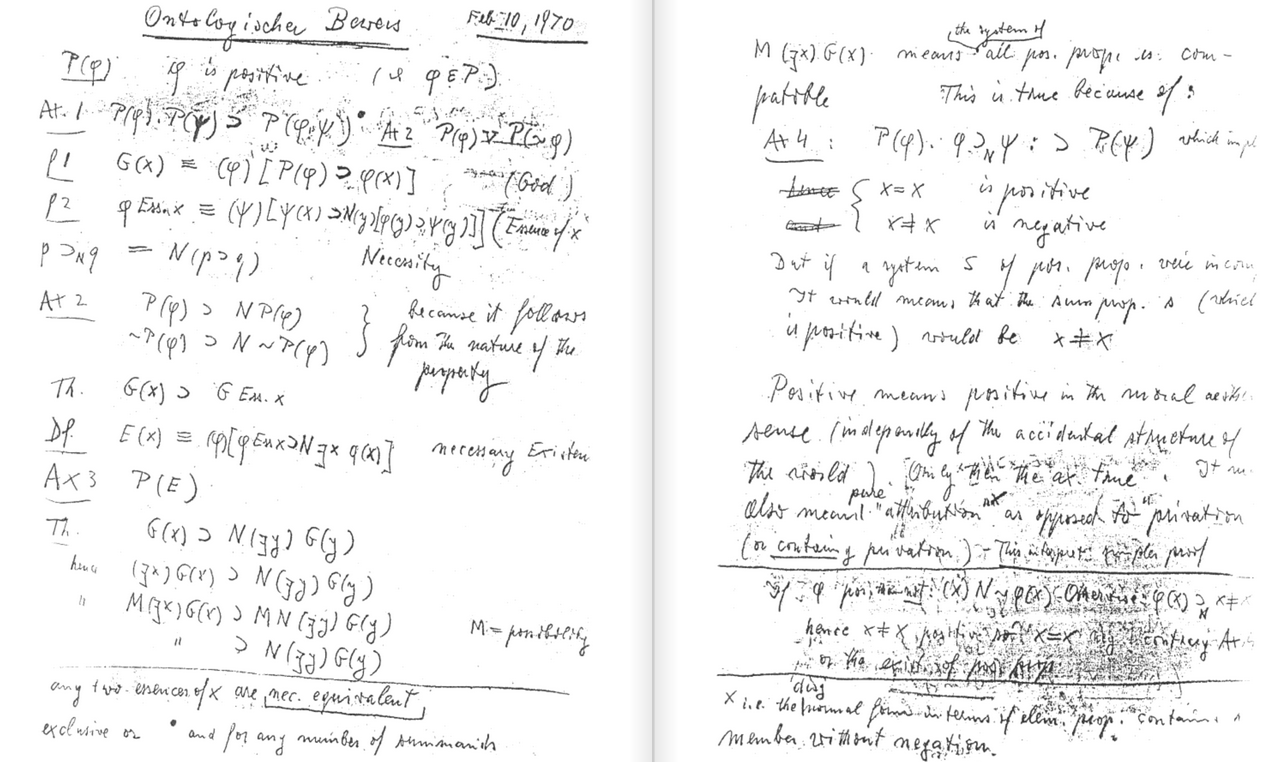
\includegraphics[width=13cm]{Images/Manuscript.png}
\end{changemargin}
\end{frame}


\begin{frame}{A Long History}{\textcolor{blue}{pros} and \textcolor{red}{cons}} \Large

\hskip-.5em
\ldots\rotatebox[origin = bl,width = 0mm]{65}{\textcolor{blue}{Anselm v. C.}} \hskip-2.3em
          \rotatebox[origin = bl]{65}{\textcolor{red}{Gaunilo}} \hskip-1.3em
\ldots  \rotatebox[origin = bl]{65}{\textcolor{red}{Th. Aquinas}}  \hskip-2.3em
\ldots\ldots   \rotatebox[origin = bl]{65}{\textcolor{blue}{Descartes}} \hskip-1.7em
               \rotatebox[origin = bl]{65}{\textcolor{blue}{Spinoza}} \hskip-1.3em
               \rotatebox[origin = bl]{65}{\textcolor{blue}{Leibniz}}  \hskip-1.2em
\ldots  \rotatebox[origin = bl]{65}{\textcolor{red}{Hume}}  \hskip-1em
          \rotatebox[origin = bl]{65}{\textcolor{red}{Kant}}  \hskip-.8em
\ldots  \rotatebox[origin = bl]{65}{\textcolor{blue}{Hegel}}  \hskip-1.3em
\ldots  \rotatebox[origin = bl]{65}{\textcolor{red}{Frege}}  \hskip-1.3em
\ldots  \rotatebox[origin = bl]{65}{\textcolor{blue}{Hartshorne}} \hskip-1.9em
          \rotatebox[origin = bl]{65}{\textcolor{blue}{Malcolm}}  \hskip-1.4em
          \rotatebox[origin = bl]{65}{\textcolor{red}{Lewis}}  \hskip-1em
          \rotatebox[origin = bl]{65}{\textcolor{blue}{Plantinga}}  \hskip-1.6em
          \rotatebox[origin = bl]{65}{\textcolor{blue}{G\"odel}}   \hskip-1.2em
\ldots \\[1em]

\pause
\vfill
Anselm's notion of God:\\
\,\hfill \emph{``God is that, than which nothing greater can be
  conceived.''} \\[1em]

G\"odel's notion of God:\\
\,\hfill \emph{``A God-like being possesses all `positive' properties.''} \\[1em]

%To show by logical reasoning: \\
%\,\hfill \emph{``(Necessarily) God exists.''} \\[1em]

\end{frame}



\begin{frame}{The Ontological Proof Today}
\vskip1em
% \emph{\huge Wohl eine jede Philosophie kreist um den ontologischen
%   Gottesbeweis} \\[1.5em]
% (Adorno, Th. W.: Negative Dialektik. Frankfurt a. M. 1966, p.378)
% \vfill
\begin{center}
\fcolorbox{gray}{white}{
\begin{minipage}{0.9\textwidth}
\hfill
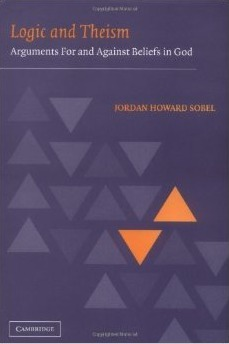
\includegraphics[height=2.2cm]{Images/Books/buch3.jpg} \hfill

\includegraphics[height=2.2cm]{Images/Books/buch2.jpg} \hfill 
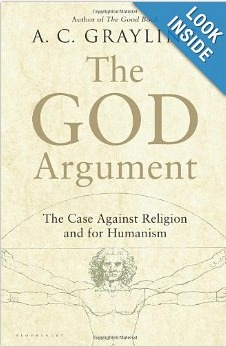
\includegraphics[height=2.2cm]{Images/Books/buch4.jpg} \hfill
\hfill

\vspace{0.5 cm}

\hfill
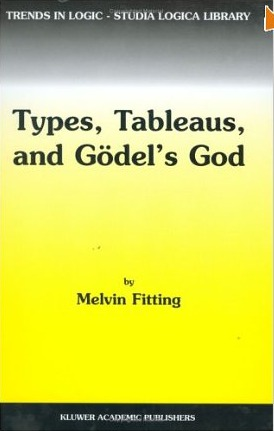
\includegraphics[height=2.2cm]{Images/Books/buch7.jpg} \hfill
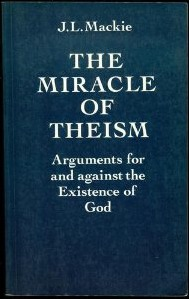
\includegraphics[height=2.2cm]{Images/Books/buch5.jpg} \hfill
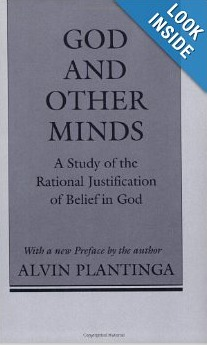
\includegraphics[height=2.2cm]{Images/Books/buch6.jpg} \hfill

\includegraphics[height=2.2cm]{Images/Books/buch1.jpg} \hfill
\hfill
\end{minipage}
}

\end{center}
\end{frame}


\begin{frame}[shrink]{Proof Overview}

$$
\textbf{D1: } G(x) \equiv \forall \varphi. [P(\varphi) \to \varphi(x)]
$$

$$
\textbf{D2: } \ess{\varphi}{x} \equiv \varphi(x) \wedge \all \psi. (\psi(x) \imp \nec \all x. (\varphi(x) \imp \psi(x)))
$$

$$
\textbf{D3: } NE(x) \equiv \all \varphi.[\ess{\varphi}{x} \imp \nec \ex y.\varphi(y)]
$$

\begin{prooftree}
\AXC{$\textbf{A3}$} \dashedLine
\UIC{$P(G)$}
		\AXC{$\textbf{A2}$} \dashedLine
		\UIC{$\all \varphi. \all \psi.[(P(\varphi) \wedge \nec \all x.[\varphi(x) \imp \psi(x)]) \imp P(\psi)]$}
					\AXC{$\textbf{A1a}$} \dashedLine
					\UIC{$\all \varphi. [P(\neg \varphi) \imp \neg P(\varphi)]$} \doubleLine
				\BIC{$\textbf{T1: } \all \varphi. [P(\varphi) \imp \pos \ex x.\varphi(x)]$} \doubleLine
	\BIC{$\textbf{C1: } \pos \ex z. G(z)$}
\end{prooftree}





\begin{prooftree}
						\AXC{$\textbf{A1b}$} \dashedLine
						\UIC{$\all \varphi. [\neg P(\varphi) \imp P(\neg \varphi)]$}
								\AXC{$\textbf{A4}$} \dashedLine
								\UIC{$ \all \varphi.[P(\varphi) \to \Box \; P(\varphi)] $} \doubleLine
							\BIC{$\textbf{T2: } \all y.[G(y) \imp \ess{G}{y}]$}
									\AXC{$\textbf{A5}$} \dashedLine
									\UIC{$ P(NE) $} \doubleLine
								\BIC{$\textbf{L1: } \ex z. G(z) \imp \nec \ex x. G(x)$} \doubleLine
								\UIC{$\pos \ex z. G(z) \imp \pos \nec \ex x. G(x)$}
										\AXC{$\textbf{S5}$} \dashedLine
 										\UIC{$ \all \xi.[\pos \nec \xi \imp \nec \xi]$} \doubleLine	
									\BIC{$\textbf{L2: } \pos \ex z. G(z) \imp \nec \ex x. G(x)$}
\end{prooftree}

\begin{prooftree}
\AXC{$\textbf{C1: } \pos \ex z. G(z)$}
		\AXC{$\textbf{L2: } \pos \ex z. G(z) \imp \nec \ex x. G(x)$} \doubleLine
	\BIC{$\textbf{T3: } \nec \ex x. G(x) $}
\end{prooftree}

\end{frame}